\section{Skaitmeninės tapatybės valdymo apžvalga}

\subsection{Tapatybės patvirtinimo poreikis}

Šiais laikais naudotojo identifikavimas yra svarbi interneto taikomųjų
programų dalis. Paslaugų tiekėjai identifikuoja savo naudotojus norėdami \cite{RalucaBudiu2014}:

\begin{itemize}
    \item registruoti (angl. \textit{log}) naudotojų veiklą,
    \item užtikrinti, kad naudotojas iš tikrųjų yra asmuo, kuris sakosi esąs,
    \item suteikti dalį funkcionalumo tik autorizuotiems naudotojams,
    \item individualizuoti tinklalapio ar taikomosios programos turinį pagal naudotojo poreikius,
    \item sukurti paslaugos naudotojų bendruomenę,
    \item išvengti galimų anoniminių naudotojų atakų.
\end{itemize}

Dėl išvardytų priežasčių naudotojų identifikavimas atlieka svarbią rolę įvairiose taikomųjų programų
srityse - elektroninėje valdžioje, elektroninėje komercijoje, verslo sumanume
(angl. \textit{business intelligence}), tyrimuose bei saugume
(angl. \textit{homeland security}) \cite{Glasser2009}. Kiekvienas paslaugų tiekėjas turi pasirinkti,
kaip autentifikuoti, ir, jei reikia, autorizuoti naudotojus. Programos kūrėjas taip pat turi užtikrinti naudotojo
suteiktų duomenų saugumą, o naudotojui tenka rūpintis skirtingų turimų
paskyrų priežiūra ir savo duomenų sklaida tarp skirtingų sistemų. Minimus tapatybės atpažinimo
skaitmeninėje erdvėje aspektus nagrinėja skaitmeninės tapatybės valdymo disciplina.

\subsection{Skaitmeninės tapatybės valdymo samprata}

Dėl nuolat vykstančios interneto ir jame esančių paslaugų plėtros tapatybių
valdymo uždavinys pastaraisiais metais tapo itin svarbus \cite{Glasser2009}. Skaitmeninės tapatybės valdymo pagrindinis uždavinys yra kontroliuoti
tapatybę ir su ja susijusius procesus, tokius kaip autentifikavimas, autorizavimas, prieigų kontrolė,
tapatybės gyvavimo ciklo valdymas bei saugus tapatybės atributų perdavimas trečiosioms šalims \cite{Cao2010, Dabrowski2008}. Sprendžiant šį uždavinį,
sukurta skirtingų skaitmeninės tapatybės valdymo sistemų. Šioms sistemoms įtaką daro
kiti tapatybę nagrinėjantys mokslai (pvz. sociologija), taip pat jos gali atlikti keletą skirtingų funkcijų, susijusių
su naudotojų tapatybe. Žemiau pateikiama diagrama,
kurioje apibendrintas tapatybės valdymo sistemų kontekstas bei pagrindinės atliekamos užduotys:

\begin{figure}[H]
    \centering
    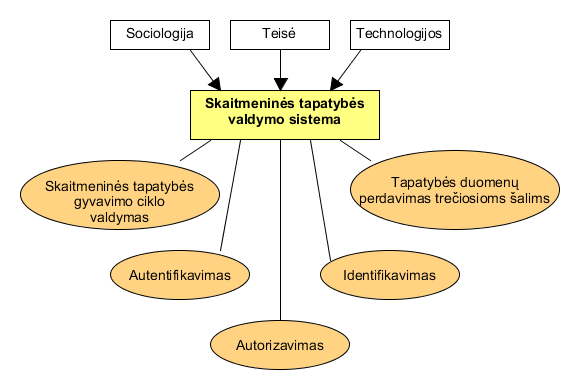
\includegraphics[scale=0.8]{img/IDMcontextAndUsecases}
    \caption{Skaitmeninių tapatybių valdymo sistemų kontekstas ir užduotys \cite{Glasser2009}}
    \label{fig:IDMContext}
\end{figure}

Paveiksle matomos disciplinos turi skirtingą poveikį tapatybių valdymo sistemoms. 
Sociologija padeda apibrėžti tapatybę ir jos atitikmenį skaitmeninėje erdvėje, teisės mokslas nusako tapatybės duomenų naudojimo reikalavimus,
o esamos technologijos formuoja sistemos įgyvendinimo niuansus. Verta pastebėti, kad tapatybės valdymo sistema gali atlikti ne visas
diagramoje nurodomas funkcijas, o tik dalį iš jų. Taip pat, ~\ref{fig:IDMContext}-ame paveiksle bei visame darbe naudojamos skaitmeninės tapatybės valdymo sąvokos,
tokios kaip \textit{identifikavimas}, \textit{autentifikavimas} ar \textit{autorizavimas} neretai suprantamos skirtingai, o tai sukelia
vieningos terminologijos trūkumą ir dėl jo kylančius neaiškumus \cite{Glasser2009}. Dėl to skyriuje
\enquote{Sąvokų apibrėžimai} pateikiami darbe naudojamų terminų aiškinimai.

Esamų tapatybių valdymo sistemų architektūros bei veikimo principai yra skirtingi -  S. Clauß ir M.Köhntopp savo tyrime pastebi,
kad nėra vieningo standarto identiteto
valdymo sistemoms \cite{Claus2001}. Tolesniuose skyriuose, apžvelgus naudotojų poreikius
tapatybės valdymo sistemoms, pateikiamos skirtingos technologijos
bei sprendimai, naudojami identiteto valdymui internete, jų privalumai bei trūkumai.

\subsection{Naudotojų poreikiai skaitmeninės tapatybės valdymo sistemoms} \label{section:IDMcharacteristics}

Skaitmeninės tapatybės valdymas yra plati sritis, kurią galima analizuoti iš skirtingų pusių: paslaugų tiekėjo, tapatybės tiekėjo ar naudotojo.
Šiame darbe į skaitmeninių tapatybių valdymą žvelgta iš naudotojo perspektyvos - kaip skaitmeninio valdymo sistemos atitinka naudotojų poreikius
bei lūkesčius. Išskirtos šios naudotojoms aktualios sistemų savybės:

% Abi pusės,
% priklausomai nuo savo poreikių, turi jiems aktualias identiteto valdymo sistemų savybes. Apžvelgiant skirtingas tapatybės valdymo sistemas,
% didžiausias dėmėsys kreiptas į naudotojams bei paslaugų tiekėjams svarbiausius sistemų bruožus.

% Tiek naudotojams, tiek paslaugų tiekėjams itin svarbus yra pasirinkto identiteto valdymo sprendimo patikimumas, t.y., asmens duomenų saugumo užtikrinimas.
% Naudotojai nenori savo asmens duomenų nutekėjimo (angl. \textit{data leakage}) internete, tuo tarpu paslaugų tiekėjai negali rizikuoti prarasti naudotojų pasitikėjimo
% jų paslauga pasirinkus nesaugų tapatybės valdymo sprendimą. Be patikimumo, naudotojams bei paslaugų tiekėjams aktualios ir 
% kitos skaitmeninio identiteto sistemų savybės. Žemiau pateikiami pagrindiniai abiejų pusių poreikiai.

\begin{itemize}
    \item identifikatorių bei slaptažodžių kiekis. Naudotojui vidutiniškai turint 25 paskyras, reikalaujančias slaptažodžių \cite{Florencio2007} bei naudojant
    nuo 2 iki 12-os el. paštų \cite{Gross2007}, jis tampa priverstas prisiminti vis daugiau identifikatorių. Atsimintinų autentifikavimo duomenų kiekiui
    augant, naudotojai yra linkę aukoti saugumą dėl patogumo ir naudoti panašius
    slaptažodžius skirtingose sistemose \cite{Pashalidis2003, Samar1999};
    \item saugumas. Privatumas yra žmogaus poreikis ir visa visuomenė nukentėtų nuo jo nebuvimo \cite{Maliki2007}.
    Suteikiant savo asmens duomenis internete naudotojai tikisi, kad jie bus patikimai
    saugomi ir nepasiekiami programišiams. Tapatybių valdymo sistemos turėtų būti budrios saugumo rizikoms bei viešai skelbti
    saugumui skirtas priemones ir atliktų saugumo analizių rezultatus, kad tiek naudotojai, tiek paslaugų tiekėjai
    galėtų pasitikėti tapatybių valdymo sistemomis \cite{Dhamija2008};
    \item asmens duomenų kontrolė. Pasak Nyderlanduose atliktų tyrimų, naudotojai nesijaučia kontroliuojantys savo asmens duomenų internete \cite{Baars2016}. Dėl to
    naudotojai pradeda nepasitikėti taikomųjų programų kūrėjais, nes jie pilnai nežino, kokia informacija apie juos kaupiama ir kokioms
    sistemoms ji perduodama;
    \item patogumas (angl. \textit{usability}). Naudotojams skaitmeninės tapatybės valdymas neretai yra tik pašalinis mechanizmas, reikalingas
    norint pasiekti paslaugą \cite{Dhamija2008}. Dėl šios priežasties sistemos naudojimosi patogumas yra svarbus - kuo tapatybės valdymas yra labiau integruotas
    su asmens jau naudojamomis sistemomis, kuo mažiau jis reikalauja papildomo naudotojo įsitraukimo ir kuo suteikia geresnę naudotojo patirtį (angl. \textit{user experience}), tuo labiau naudotojas bus linkęs pasirinkti šį identiteto valdymo sprendimą.
\end{itemize}

% \chapter{\textbf{Paslaugų tiekėjams aktualios tapatybės valdymo sistemų savybės:}}

% \begin{itemize}
%     \item kaštai, skirti tapatybės valdymui. Priklausomai nuo pasirinkto sprendimo,
%     paslaugų tiekėjui gali tekti skirti daug arba mažai resursų (programuotojų, laiko, investavimo į technologijas)
%     naudotojų tapatybės valdymo veiksmams užtikrinti;
%     \item naudotojo patirties kontrolė (angl. \textit{user experience control}). Paslaugų tiekėjai siekia užtikrinti teigiamą
%     naudotojų patirtį dėl geresnio naudojamumo, privatumo ir saugumo \cite{Dhamija2008}, o tapatybės valdymo sistemos veikimo primesti sprendimai (pvz. nukreipimai į kitą tinklalapį) gali daryti
%     tam įtaką.
% \end{itemize}

\subsection{Esamos skaitmeninių tapatybių valdymo sistemos}

Tapatybių valdymo sistemos yra pagrįstos skirtingomis architektūromis, kurios įgalina
konkrečios sistemos veikimą. Šiame skyriuje tiriami 3-ys dažniausiai naudojami identiteto valdymo
modeliai. Tiriant kiekvieną modelį, pirmiausia apžvelgti jo bendri veikimo principai. Toliau, apžvelgtos paplitusios modelio realizacijos, kurių technologiniai
sprendimai gali turėti įtakos naudotojų poreikiams. Galiausiai, analizuotas sistemos atitikimas naudotojų lūkesčiams,
išvardytiems \ref{section:IDMcharacteristics} skyrelyje.

\subsubsection{Izoliuotas tapatybių valdymas}

\subsubsubsection*{Modelis}

Izoliuotame modelyje paslaugų tiekėjas yra ir tapatybės tiekėjas, nes visos su tapatybės valdymu
susijusios operacijos yra atliekamos vieno serverio. Tapatybės duomenų saugojimas, autentifikavimas
ir autorizavimas yra įgyvendinti paties paslaugų tiekėjo \cite{Cao2010}. Kiekvienas naudotojas turi atskirus identifikatorius
kiekvienai naudojamai paslaugai. Modelis grafiškai pavaizduotas žemiau esančiame paveiksle:

\begin{figure}[H]
    \centering
    \includegraphics[scale=0.65]{img/IsolatedModel}
    \caption{Izoliuotas skaitmeninės tapatybės valdymas \cite{Cao2010}}
\end{figure}

Pagal izoliuotą modelį, naudotojas turi savo paskyrą kiekvienoje naudojamoje sistemoje. Kiekvieną kartą autentifikuojant ar autorizuojant
naudotoją, tai atlieka pats paslaugų tiekėjas, bendraudamas tiesiogiai su naudotoju (jo naršykle). Naudotojui prisijungus prie vieno tinklalapio ir gavus
prieigos raktą, jis gali toliau naudotis šiuo tinklalapiu, tačiau prireikus pasinaudoti kita taikomąja programa, tapatybės atpažinimo veiksmai (autentifikavimas, autorizavimas)
turi vėl būti atlikti naujoje sistemoje.

\subsubsubsection*{Realizacijos}

Kadangi šis naudotojų autentifikavimo bei autorizavimo modelis naudojamas seniausiai,
yra gana nemažai jį įgyvendinusių taikomųjų programų. Lietuvoje šį modelį naudoja
\enquote{Tiketa}, \enquote{Bilietai.lt}, \enquote{Pigu.lt},
\enquote{Varle.lt}, pasaulyje - \enquote{Booking.com}, \enquote{Skycop}, \enquote{AirBnB} bei kitos platformos. Verta
pastebėti, kad dalis iš jų jau remiasi ne vien tik savo izoliuotu tapatybės valdymu, bet jau turi į savo sistemas integravę ir papildomų autentifikavimo būdų
(pvz. prisijungimą per \enquote{Facebook} ar \enquote{Google}).

Realizacijų technologiniai sprendimai dažniausiai nėra viešai prieinami.
Šiame modelyje kiekvienas paslaugų tiekėjas yra ir tapatybės tiekėjas, tad nereikia
apibrėžti protokolų, duomenų formatų ar kitų detalių, kurios formalizuotų bendravimą tarp pasikliaujančiosios šalies ir
tapatybės tiekėjo - visa tai pats nusprendžia ir įgyvendina paslaugų tiekėjas.

\subsubsubsection*{Patrauklumas naudotojams}

Nors izoliuotas tapatybių valdymas yra gana paprastas paslaugų tiekėjams, tačiau jis greitai tampa
nebekontroliuojamu naudotojams \cite{Josang2005}. Jis verčia naudotojus turėti paskyrą kiekvienai paslaugai, o tai lemia
daugybės identifikatorių ir slaptažodžių valdymą. Tai sukelia \enquote{slaptažodžių nuovargį} (angl. 
\textit{password fatigue}), kas veda prie tų pačių identifikatorių ir slaptažodžių pasirinkimo skirtingoms paslaugoms \cite{Dhamija2008}.

Izoliuotame identiteto valdyme programišiams sunkiau atlikti sukčiavimo (angl. \textit{phishing}) ataką, nes naudotojas
nebūna nukreipiamas į tapatybės tiekėjo puslapį. Tai pagerina šio modelio saugumą. Dėl to, kad paslaugų tiekėjas yra ir tapatybės tiekėjas,
šiame modelyje galima išvengti duomenų perdavimo tarp skirtingų serverių - tokiu būdu sumažėja ir rizika, kad šiuos duomenis
jų persiuntimo metu perims programišius. Tačiau, standartų duomenų formatams bei perdavimui nebuvimas gali paskatinti paslaugų
tiekėjus nepažvelgti į tai atsakingai ir įgyvendinti bendravimą su naudotojo naršykle atmestinai.

Naudotojų asmens duomenų kontrolė šiame modelyje priklauso nuo kiekvienos paslaugos. Asmenys atskirai suteikia savo duomenis
kiekvienai paslaugai, dažniausiai paskyros sukūrimo metu. Jei paslauga informuoja apie duomenų panaudos atvejus (pvz. kam bus naudojamas
el. pašto adresas), tuomet asmuo jausis labiau užtikrintas savo duomenų kontrole. Tačiau dėl šiame modelyje neišvengiamo duomenų suteikimo
dideliam skirtingų paslaugų kiekiui, asmeniui tampa sunku prisiminti kiekvienos naudojamos platformos duomenų platinimo taisykles.

Izoliuotame tapatybės valdyme naudotojams tenka kartoti identifikavimo procesus (autentifikavimą, autorizavimą) tiek kartų, kiek paslaugų siekiama
naudotis. Tai vargina naudotojus ir kuria blogą naudotojo patirtį. Tačiau, izoliuotas tapatybės valdymas pasižymi nuoseklia vartotojo sąsaja (dėl 
visų tapatybės valdymo procesų įgyvendimo tame pačiame paslaugų tiekėjo puslapyje), tad tai šiek tiek pagerina bendrą naudotojo patirtį.

\subsubsection{Centralizuotas tapatybių valdymas}

\subsubsubsection*{Modelis}
Centralizuotame skaitmeninių tapatybių valdyme egzistuoja vienas tapatybės tiekėjas, į kurį kreipiasi visos paslaugos,
esančios to paties paslaugų tiekėjo domene \cite{Josang2005}. Paslaugų tiekėjo ir tapatybės tiekėjo funkcijos tampa atskirtos - 
tapatybės tiekėjas rūpinasi naudotojo identiteto valdymu, o paslaugų tiekėjas koncentruojasi į paslaugos vystymą. Kai paslaugų tiekėjui
reikia autentifikuoti naudotoją (ar atlikti kitą tapatybės valdymo procesą), jis persiųs naudotojo įvestą informaciją (pvz. identifikatorių) tapatybės tiekėjui,
siekdamas pabaigti procesą \cite{Cao2010}. Naudotojui šiame modelyje užtenka vieno identifikatoriaus ir slaptažodžio, su kuriais jis gali prisijungti prie visų to paties
paslaugų tiekėjo paslaugų.

Šis modelis iliustruotas ~\ref{fig:isolatedModel}-iame paveiksle.



\begin{figure}[H]
    \centering
    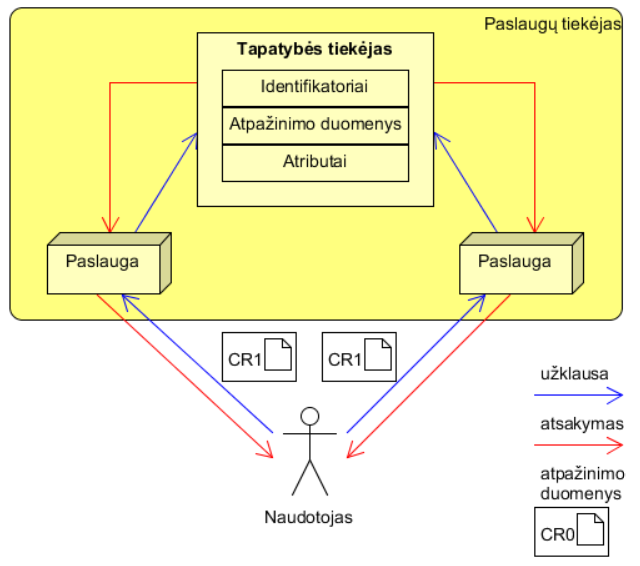
\includegraphics[scale=0.8]{img/centralizedModel}
    \caption{Centralizuotas skaitmeninės tapatybės valdymas \cite{Cao2010}}
    \label{fig:isolatedModel}
\end{figure}

\textcolor{red}{jei reik, pastraipa paslaugų tiekėjo bruožams}.

\subsubsubsection*{Realizacijos}

Centralizuotas modelis tinkamas naudoti vieno paslaugų tiekėjo ribose \cite{Josang2005}. Vienas iš pavyzdžių - 
\enquote{Atlassian} įmonės paslaugos. Naudotojui pakanka turėti vieną \enquote{Atlassian} paskyrą ir jis gali naudotis
skirtingais šio paslaugų tiekėjo produktais, tokiais kaip \enquote{Jira}, \enquote{Confluence}, \enquote{Bitbucket} bei kitais. \enquote{Atlassian}
turi ir vienkartinio prisijungimo sąlygas - paslaugas galima sukonfigūruoti taip, kad prisijungus prie vienos iš jų,
naudotojas automatiškai tampa prisijungęs ir prie kitų paslaugų.

\textcolor{red}{pridėt Kerberos}

\subsubsubsection*{Patrauklumas naudotojams}
 
Iš naudotojo perspektyvos, šis modelis yra patogesnis nei izoliuotas. Naudotojui pakanka turėti vieną identifikatorių,
kuris bus tinkamas visoms paslaugoms. Priklausomai nuo realizacijos, naudotojui gali tekti iš naujo prisijungti prie kiekvienos
paslaugos arba vieną kartą prisijungti prie betkurios iš paslaugų ir tapti autentifikuotu visose kitose paslaugose \cite{Josang2005}. Naudotojo asmens
duomenų kontrolė yra geresnė nei izoliuotame skaitmeninės tapatybės valdyme, nes naudotojas asmens duomenis patiki mažesniam kiekiui esybių
(vietoj kiekvienos paslaugos, kiekvienam paslaugų tiekėjui).

Pagrindinis šio modelio trūkumas yra tas, kad jis galimas naudoti tik vieno paslaugų tiekėjo srityje (angl. \textit{scope}). Tai palieka laisvės paslaugų tiekėjui tapatybės valdymo sistemos
realizavimui (tai gali būti centralizuota platforma įmonės ribose), tačiau naudotojas negali turimo identifikatoriaus
naudoti kito paslaugų tiekėjo sistemose.

\subsubsection{Jungtinis tapatybių valdymas}


\subsubsubsection*{Modelis}

Centralizuotas modelis reikalauja visų naudotojų būti tame pačiame domene, tačiau naudotojams reikia
paslaugų ir iš kitų domenų \cite{Cao2010}. Jungtinis (angl. \textit{federated}) tapatybių valdymas yra aibė technologijų
ir procesų, kurie leidžia sistemoms dalintis tapatybės informacija ir deleguoti tapatybės valdymo užduotis
tarp skirtingų paslaugų tiekėjų \cite{Maler2008}. Šis tapatybių valdymo modelis įgalina naudotojus turėti vieną
identifikatorių, kurį gali naudoti skirtingų paslaugų tiekėjų tinklalapiuose. Žemiau pateikiama schema, nusakanti
šio modelio architektūrą:

\begin{figure}[H]
    \centering
    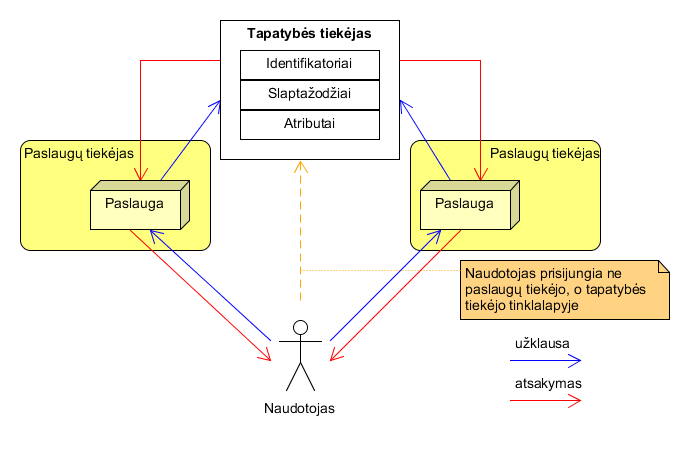
\includegraphics[scale=0.75]{img/federatedModel}
    \caption{Jungtinis skaitmeninės tapatybės valdymas \cite{Cao2010}}
    \label{fig:federatedModel}
\end{figure}

Jungtiniame tapatybės valdyme tapatybės tiekėjas yra atskira sistema, su kuria turi integruotis paslaugų tiekėjas. Tapatybės
duomenys bei su tapatybe susiję veiksmai (autentifikavimas, autorizavimas) yra deleguojami šiai sistemai. Naudotojas turi vieną identifikatorių,
su kuriuo prisijungia tiesiogiai tapatybės tiekėjo puslapyje. Prisijungus šioje sistemoje, naudotojas tampa
autentifikuotas visose paslaugose, kurios palaiko šį tapatybės tiekėją \cite{Maler2008}.

Šis tapatybių valdymo modelis yra gana patogus naudotojams. Jiems užtenka turėti vieną identifikatorių, su kuriuo
gali prisijungti prie tinklalapių iš skirtingų paslaugų tiekėjų. Asmens duomenų saugumas priklauso nuo
bendravimo tarp paslaugų bei tapatybės tiekėjų, o šiame modelyje jis sudėtingesnis nei izoliuotame ar centralizuotame
tapatybių valdyme, nes jungtinis valdymas paremtas tarpdomeniniu bendravimu \cite{Maler2008}. Naudotojo duomenų kontrolė jungtiniame 
modelyje turi tiek privalumų, tiek trūkumų. Viena vertus, naudotojas savo asmens duomenis suteikia mažesniam kiekiui sistemų (tik tapatybės tiekėjams,
vietoj visų paslaugų tiekėjų). Tačiau taip paslaugų tiekėjas tampa vieninteliu nesekmės tašku (angl. \textit{single point of failure}) - programišiams įsilaužus
į tapatybės tiekėjo sistemą, asmens paskyros visose paslaugose tampa prieinamos \cite{Pashalidis2003}. Taip pat, naudotojui gali būti sunku kontroliuoti
savo duomenų sklaidą tarp tapatybės tiekėjo ir skirtingų paslaugų, ką rodo ir \textit{Cambridge Analytica} incidentas \cite{CambridgeAnalytica}.

\textcolor{red}{jei reik, pastraipa paslaugų tiekėjo bruožams}.

\subsubsubsection*{Realizacijos}

\textcolor{red}{paimt iš kursinio}

\subsection{Tapatybių valdymo sistemų palyginimas}

% Please add the following required packages to your document preamble:
% \usepackage{multirow}
% \usepackage{graphicx}
\begin{table}[h]
    \centering
    \caption{My caption}
    \label{my-label}
    \resizebox{\textwidth}{!}{%
    \begin{tabular}{|l|l|l|l|l|l|}
    \hline
    \multicolumn{1}{|c|}{\multirow{2}{*}{Modelis}} & \multicolumn{1}{c|}{\multirow{2}{*}{\begin{tabular}[c]{@{}c@{}}Identifikatorių\\ kiekis\end{tabular}}} & \multicolumn{3}{c|}{Patogumas} & \multicolumn{1}{c|}{\multirow{2}{*}{\begin{tabular}[c]{@{}c@{}}Asmens duomenų\\ kontrolė\end{tabular}}} \\ \cline{3-5}
    \multicolumn{1}{|c|}{} & \multicolumn{1}{c|}{} & \multicolumn{1}{c|}{\begin{tabular}[c]{@{}c@{}}Prisijungimų\\ kiekis\end{tabular}} & \multicolumn{1}{c|}{\begin{tabular}[c]{@{}c@{}}Papildoma programinė\\ įranga\end{tabular}} & \multicolumn{1}{c|}{Naudotojo patirtis} & \multicolumn{1}{c|}{} \\ \hline
    Izoliuotas &  &  &  &  &  \\ \hline
    Centralizuotas &  &  &  &  &  \\ \hline
    Jungtinis &  &  &  &  &  \\ \hline
    \end{tabular}%
    }
\end{table}